%% Included in decks: slidemage-manual
%%

% SlideMage manual, chapter "Working in SlideMage": the main window, with
% numbered callouts drawn over the screenshot (positions as fractions of the
% image, so they stay put if the image is resized).
\providecommand{\callout}[2]{\node[circle, fill=c_primary_highlight, text=white, inner sep=1pt, minimum size=9pt, font=\tiny\bfseries] at (#1) {#2};}
\begin{standardframe}{The main window}
	\begin{columns}[T,onlytextwidth]
		\begin{column}{0.66\linewidth}
			\begin{tikzpicture}
				\node[anchor=south west, inner sep=0pt] (shot) at (0,0) {\setlength{\fboxsep}{0pt}\fcolorbox{c_primary_gray}{white}{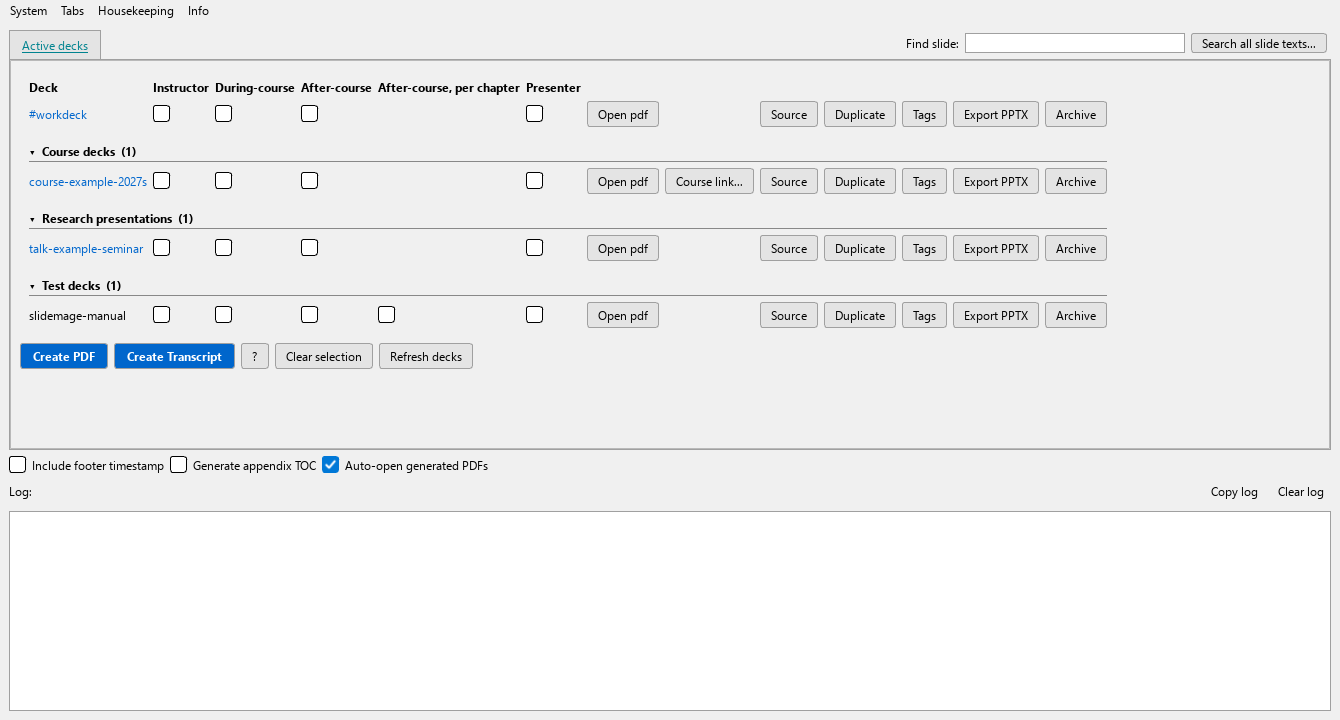
\includegraphics[width=\dimexpr\linewidth-0.8pt\relax]{media/screenshot-slidemage-main-window.png}}};
				\begin{scope}[x={(shot.south east)}, y={(shot.north west)}]
					% beside each element (tools/manual/make_screenshots.py prints
					% the elements' centres; screenshot 1340 x 720 px, 2026-10-05)
					% (a callout must stay inside the picture: one past its edge
					% widens the column -- overfull box)
					\callout{0.190,0.986}{1}
					\callout{0.090,0.939}{2}
					\callout{0.080,0.879}{3}
					\callout{0.845,0.749}{4}
					\callout{0.048,0.452}{5}
					\callout{0.400,0.354}{6}
					\callout{0.500,0.151}{7}
					\callout{0.645,0.940}{8}
				\end{scope}
			\end{tikzpicture}
		\end{column}
		\begin{column}{0.31\linewidth}
			\footnotesize
			One row per deck: tick the versions you want and press \emph{Create PDF}.
			\par\smallskip
			\scriptsize
			\begin{enumerate}
				\item Menus: settings, project, housekeeping
				\item Tabs; editors open here
				\item A checkbox per deck version
				\item PDF, course link, source, copy, tags, PowerPoint, archive
				\item \emph{Create PDF}: compile what is ticked
				\item Footer timestamp; appendix
				\item The compile log
				\item \emph{Find slide}; search all texts
			\end{enumerate}
		\end{column}
	\end{columns}
\end{standardframe}
